\ylDisplay{Klaaskuulike} % Ülesande nimi
{Jaan Kalda} % Autor
{lahtine} % Voor
{2010} % Aasta
{G 4} % Ülesande nr.
{4} % Raskustase
{
% Teema: Geomeetriline-optika
\ifStatement
Paljudes helkurmaterjalides kasutatakse valguse tagasisuunamiseks tillukesi
klaaskuulikesi, mis kantakse tiheda kihina materjali pinnale. Uurigem, milline
peaks olema selliste klaaskuulikeste murdumisnäitaja. Teeme järgmised eeldused:
(a) klaaskuulile langeb valguskiir nii, et valguskiire ja pinnanormaali vaheline
nurk $\alpha$ on väike ($\alpha \ll \SI{1}{rad}$); (b) valguskiir murdub klaasi
pinnal, peegeldub ühekordselt kuuli sisepinnalt ja väljub seejärel kuulist
(murdudes teistkordselt kuuli pinnal). Millise murdumisnäitaja $n$ korral
suundub selline valguskiir täpselt tagasi? Tehke kiirtekäigu joonis ja
põhjendage vastust. \emph{Abivalem:} väikese $\alpha$ korral radiaanmõõdus
$\sin\alpha \approx \alpha$.
\fi


\ifHint
Ülesande mugavamaks lahendamiseks tuleb teha selge joonis ning rakendada väikeste nurkade lähendust. Lisaks, kiire ja kuuli puutepunkti pinnanormaal ühtib kuuli raadiusega.
\fi


\ifSolution
Tagasipeegelduv kiir peegeldub kuulikeses nii, nagu näidatud joonisel. Murdumisseadusest väikeste nurkade jaoks saame
$n=\sin 2\alpha/\sin\alpha \approx 2.$
\begin{center}
	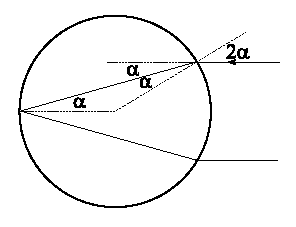
\includegraphics[width=0.35\textwidth]{2010-lahg-04-kuulike.eps}
\end{center}
\fi
}